\clearpage
\title{Problem 4.2}
\author{}
\date{}
\maketitle

\section*{Problem Description}
Write a program to display a "?", read two capital letters, and display them on the next line in alphabetical order.

\section*{Process}
\subsection*{Code:}

\begin{multicols}{2}{|}
    \begin{minted}[linenos,breaklines,breakanywhere]{nasm}
DATA SEGMENT
    CR EQU 0DH
    LF EQU 0AH
    MSG1 DB CR, LF, '? $'
    CHAR1 DB ?
    CHAR2 DB ?
DATA ENDS  

CODE SEGMENT
    ASSUME CS:CODE, DS:DATA

START:
    LEA DX, MSG1
    MOV AH, 9
    INT 21H
    
    MOV AH, 1 
    INT 21H
    MOV CHAR1, AL
    
    MOV AH, 1
    INT 21H
    MOV CHAR2, AL
    
    MOV AL, CHAR1
    MOV BL, CHAR2
    
    CMP AL, BL
    JLE SKIP_SWAP
    MOV CHAR1, BL
    MOV CHAR2, AL
    
SKIP_SWAP:
    ; newline
    MOV AH, 2
    MOV DL, 0Dh
    INT 21h
    MOV DL, 0Ah
    INT 21h
    
    ; first character
    MOV AH, 2
    MOV DL, CHAR1
    INT 21h
    
    ; second character
    MOV AH, 2
    MOV DL, CHAR2
    INT 21h
    
    ; Terminate program
    MOV AH, 4Ch
    INT 21h 
    
CODE ENDS

END START
\end{minted}
\end{multicols}

\subsection*{Output}
\begin{center}
    \centering
    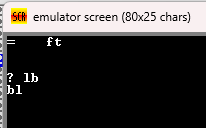
\includegraphics[width = .4\textwidth]{2.png}
    \captionof{figure}{Ordering letters alphabetically}
\end{center}


